\documentclass[UTF8]{ctexart}
\usepackage{ctex}
\usepackage{geometry}
\usepackage{enumitem}
\usepackage{indentfirst}
\usepackage{color}
\usepackage{fancyhdr}
\usepackage{amsmath}
\usepackage{graphicx}
\usepackage{amssymb}
\usepackage{tikz}
\usepackage{cases}
\usepackage{array}
\usepackage{pgfplots}
\usepackage{tkz-euclide}

% 设置纸张和页边距——A4
\geometry{papersize={21cm,29.7cm}}
\geometry{left=3.18cm,right=3.18cm,top=2.54cm,bottom=2.54cm}

% 一级标题靠左
\CTEXsetup[format={\Large\bfseries}]{section}

% 去除页眉
\pagestyle{plain}

%设置段间距
\addtolength{\parskip}{.4em}
%%设置行间距
%\usepackage{setspace}
%\setstretch{2.5}

% 开始文档内容
\begin{document}

\title{信号与系统课程笔记:Lecture 11,傅里叶变换(Fourier Transform) }
\author{授课教师:秦雨潇 \\
        笔记记录:曹时成}
\date{2023 年 10 月 25 日(第八周,周三)}
\maketitle

\section{课堂回顾}
$f(t)=\sum_{n=-\infty}^{+\infty}F[\omega]e^{j\omega{t}}\qquad$ $n\in \mathbb{Z}$ ,$\omega=n\Omega=n\frac{2\pi}{T}  $ \par
$F[\omega]=\frac{1}{T}\int_{-\frac{\pi}{2}}^{\frac{\pi}{2}}f(t)e^{-j\omega{t}}{\rm{dt}}$ \par
\section{答疑}
相关度衡量两个信号之间的相似性或关联性,\textbf{而不要求其中一个信号经过翻转(卷积要求一个信号经过翻转)。}相关可以是自相关(一个信号与自己的相关)或互相关(两个不同信号之间的相关)。\par
卷积:convolution \par
互相关:cross-Correlation \par
\begin{figure}[h]
    \centering         %使图片居中放置
    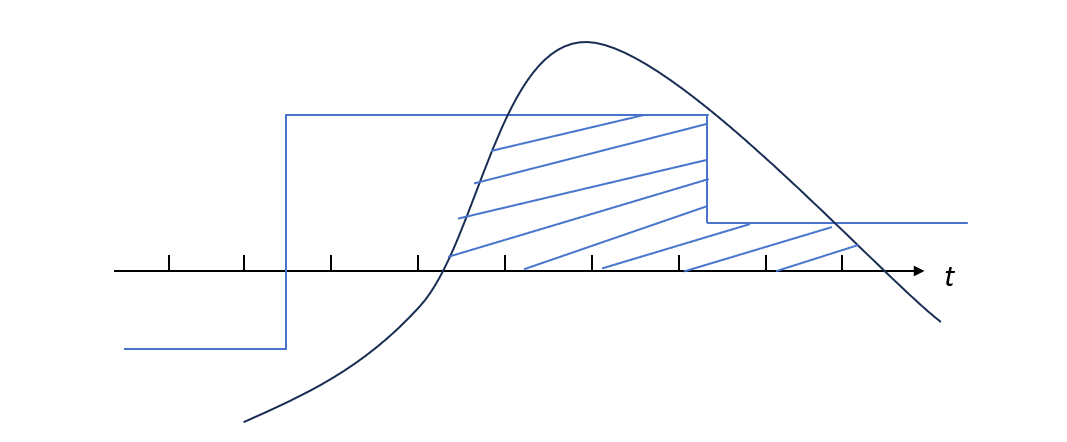
\includegraphics[scale=0.5]{1.jpg}
    \caption{互相关示意图}
\end{figure}
\; \par
\; \par
\; \par
自相关:Auto-correlation \par
\begin{figure}[h]
    \centering         %使图片居中放置
    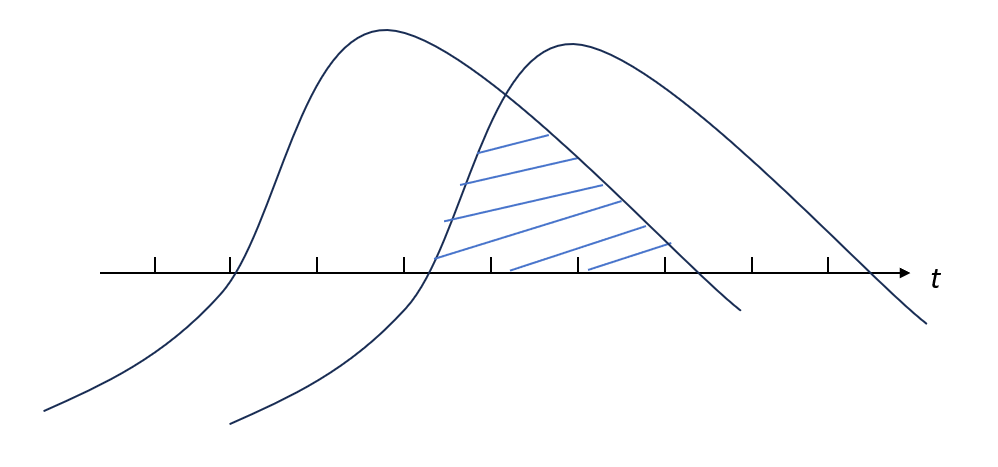
\includegraphics[scale=0.5]{2.png}
    \caption{自相关示意图}
\end{figure}
\section{傅里叶变换实例演示}
\subsection{键盘声音的频谱演示}
\subsection{短视频:用乐器演示声音在频谱上的变化}
\subsection{编程实现对一段音频的傅里叶变换并演示信号的拉伸与压缩}
(1)信号在时域的拉伸对应着在频域上的压缩 \par
\begin{figure}[h]
    \centering         %使图片居中放置
    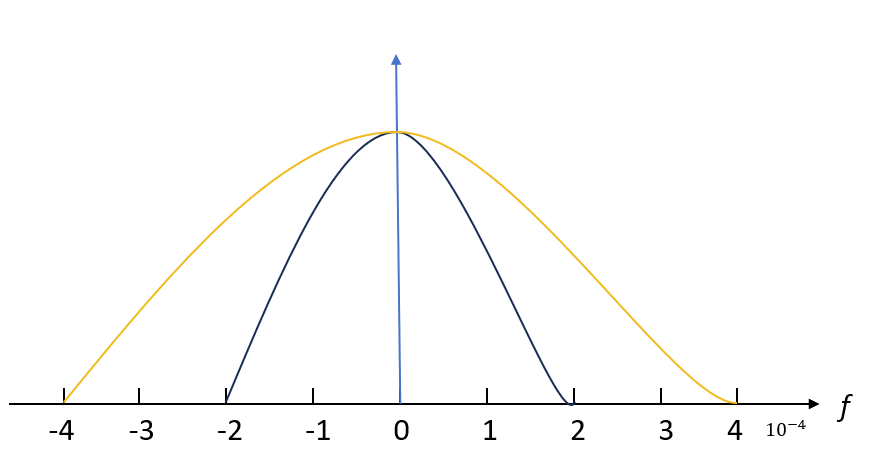
\includegraphics[scale=0.5]{3.png}
    \caption{信号在频域的拉伸}
\end{figure}
思考:信号在频谱上进行压缩,压缩前超过 $\pm 40000$  Hz 的信号在压缩后去哪了?\par
(2)信号在时域的压缩对应着在频域上的拉伸\par
信号如何拉伸,是关于采样定理部分的内容 \par
思考:信号在频谱上进行拉伸,拉伸前超过 $\pm 20000$  Hz 的信号在拉伸后后去哪了?\par
\end{document}